\documentclass[11pt]{article}
\usepackage[english]{babel}
\usepackage[utf8]{inputenc}
\usepackage{fancyhdr}
\usepackage{graphicx}
\usepackage{wrapfig}
\usepackage{amssymb}
\usepackage{float}
\usepackage[table,xcdraw]{xcolor}
\usepackage{blindtext}
\usepackage{setspace}
\usepackage{listings}
\usepackage[
backend=biber,
style=mla-new,
citestyle=authoryear
]{biblatex}
\addbibresource{sources.bib}

\usepackage{geometry}
 \geometry{
 a4paper,
 left=20mm,
 right=20mm,
 bottom=25mm,
 top=25mm,
 }

\pagestyle{fancy}
\fancyhf{}
\lhead{Research Question: How does the mass of a Tuned Mass Damper affect the dissipation of mechanical energy in an oscillating structure? }
\rfoot{Page \thepage}

\title{Fighting earthquakes with pendulums: the Tuned Mass Damper}

\author{Physics Internal Assessment}

\date{September 2021}


\begin{document}
\begin{titlepage}
	\centering
	{\huge\bfseries Fighting Earthquakes with Pendulums: the Tuned Mass Damper \par}
	\vspace{2cm}
	{\scshape\Large Research Question: How does the mass of a Tuned Mass Damper affect the dissipation of mechanical energy in an oscillating structure? \par}
	\vspace{1.5cm}
	{\Large\itshape Physics Internal Assessment \par}
	\vspace{0.5cm}
	{\Large\itshape IB Number: CENSORED \par}

	\vfill

% Bottom of the page
\end{titlepage}


\clearpage
\section{Introduction}

19th of September, 1985: Mexico City was shaken to the ground by an 8.0 Mw earthquake, buildings collapsing onto citizens totalling 5,000 deaths. 19th of September, 2017: Mexico City was hit again by a 7.1 Mw earthquake; however, despite more skyscrapers towering over the city skyline than in 1985, they did not collapse \autocite{vance}. As the ground was shaking beneath my feet, my safety and that of countless Mexicans trapped in swaying towers were rescued by the physics of damping mechanisms. One such damping mechanism is called a Tuned Mass Damper, which is a “system for damping the amplitude in one oscillator by coupling it to a second [damped] oscillator” causing energy from the earthquake to be “‘transferred’ to the second oscillator” \autocite{orloff}. Given their rarity in industrial skyscrapers, I wanted to investigate the effectiveness of a pendulum TMD in combating earthquakes like the ones I experienced in Mexico. However, I discovered that architects often chose lighter dampers to save costs, leading to very little research on what the mass of a TMD should be to most effectively dampen oscillation. Hence, I decided to investigate the effect of mass on the dampening of the structure by asking the research question: \textbf{How does the mass of a Tuned Mass Damper affect the dissipation of mechanical energy in an oscillating structure?}

\section{Theoretical Background}

\begin{wrapfigure}{l}{0.2\linewidth}
\vspace{-15pt}
\centering
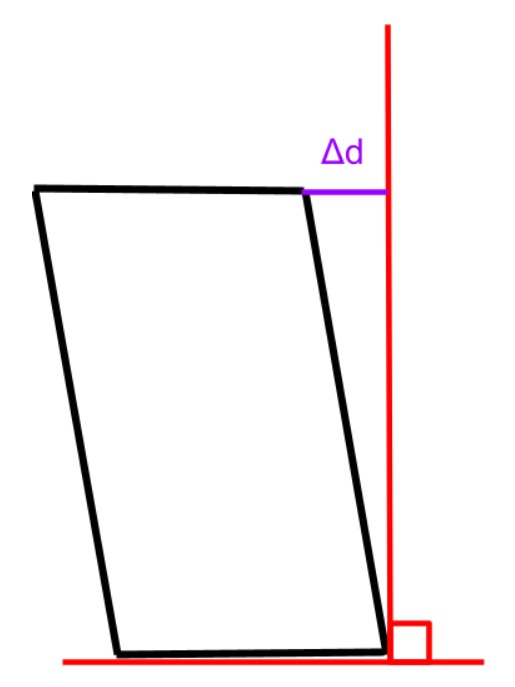
\includegraphics[width=0.2\textwidth]{img/fig1.jpg}
\caption{\label{fig:1}Initial displacement}
\vspace{-50pt}
\end{wrapfigure}

This investigation consists of three components: the earthquake, the structure, and the pendulum Tuned Mass Damper.

\subsection{The Earthquake}

An earthquake repeatedly displaces the base of a structure ("How Do..."). Changing points of reference, it displaces the top of the structure by $\Delta d$ (meters) as seen in Figure 1. Simulating this effect, I will simplify the impact of an earthquake on a structure as a single initial displacement $\Delta d_1$, after which no external force will be applied.


\subsection{The structure}

Internal reinforcement of the structure applies a restoring force, $F_s$ (Newtons), to bring the structure back to vertical equilibrium, a force denoted by $F_s \propto -\Delta d$. A force opposite and proportional to displacement oscillates the structure around its equilibrium, denoted by the vertical red line in Figure 2, resulting in simple harmonic motion.



\subsection{The Dampening}

\begin{wrapfigure}{l}{0.6\linewidth}
\centering
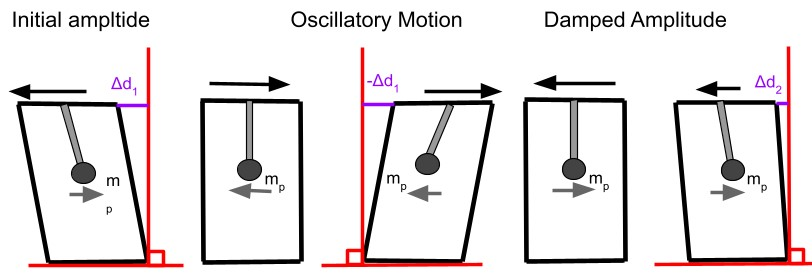
\includegraphics[width=0.6\textwidth]{img/fig2.jpg}
\caption{\label{fig:2}Animation frame of damping oscillation}
\vspace{-10pt}
\end{wrapfigure}

As the structure oscillates, some of its mechanical energy, $ME$ (Joules), is transferred into other forms of energy (eg. thermal energy) causing each successive amplitude (meters) of the structure’s oscillation to be smaller than the previous one, known as damping as visualized in Figure 2. Now consider a pendulum at the top of the structure, the TMD. When it oscillates due to the displacement of the top of the structure, it transfers energy from the structure into its own oscillation \autocite{connor}. This occurs because the pendulum absorbs some of the structure's mechanical energy in order to oscillate itself. Due to the additional damping of the TMD (caused by friction in the rotating hinge of the pendulum), it further dampens the structure’s oscillation, meaning that the consecutive maximum displacement of the structure, $\Delta d_2$ (meters) will be lower than $\Delta d_1$ (meters). Similarly, the mechanical energy of the structure during the second period of oscillation will be smaller than the initial mechanical energy, $ME_2 < ME_1$, because of the dissipation of mechanical energy caused by the TMD. The mass of the pendulum, $m_p$ (grams) will be modified to measure the effect on damping between $ME_1$ and $ME_2$.

\section{Deriving The Formula}

To measure the total mechanical energy in the oscillating structure, I can use $ME=\frac{1}{2}k\Delta d ^2+\frac{1}{2}mv_2$ (Joules), the sum of its kinetic and potential energy, with some unknown constant $k$, mass $m$, and velocity $v$. However, at maximum displacement $\Delta d_1$ and $\Delta d_2$, there is no kinetic energy, simplifying the equation to $ME=\frac{1}{2}k \Delta d^2$. To measure the percentage loss of mechanical energy due to damping, we can use the equation $$\frac{ME_1-ME_2}{ME_1}\times100\%$$ which cancels out the unknown constant $\frac{1}{2}k$ resulting in the neat formula $\zeta=\frac{\Delta d_1^2-\Delta d_2^2}{\Delta d_1^2}\times100\%$ where $\zeta$ (\%) is the percentage of lost mechanical energy.
$\Delta d_1$ is a constant variable, equal to the initial displacement of the structure as a result of the earthquake. $\Delta d_2$ is the maximum displacement of the structure during its second period of oscillation, which allows me to measure the immediate loss in mechanical energy between the first two consecutive periods of oscillation. I can not measure $\Delta d_2$ in meters because it oscillates too fast for a human to measure, which is why I will use an accelerometer. The relationship between acceleration and displacement is $a=\omega ^2 \Delta d$ where $\omega=2\pi f$, where $f$ is a constant, representing the frequency of the building’s oscillation. I can therefore use $$\Delta d_2=\frac{a_2}{4\pi^2f^2}$$ where $a_2$ is the maximum acceleration of the structure in the second period of oscillation. This results in the final equation for $\zeta$ (Equation 1, \% of ME lost between first two consecutive periods) as:

\begin{equation}
    \label{eqn:zeta}
    \zeta=\frac{\Delta d_1^2-(\frac{a_2}{4\pi^2f^2})^2}{\Delta d_1^2} \times 100\%
\end{equation}

\section{Hypothesis}
I hypothesise that the percentage loss in mechanical energy $\zeta$ (\%) increases linearly as $m_p$ increases because the larger mass of the Tuned Mass Damper can absorb more kinetic energy, since kinetic energy is dependent on mass, as seen in the formula $KE_p=\frac{1}{2}m_pv^2$. Hence, this could achieve the relationship $\zeta \propto m_p$ where the mass is proportional to the percentage of mechanical energy dissipated.

\section{Setting up the Experiment}

I had to build the structure using only materials in my garage while maintaining the rigidity-flexibility and height-width ratio of a real skyscraper. I approximated this by attaching plastic straws to each other with toothpicks totalling $30cm$ high. They are attached to $5cm x 5cm$ wooden planks. For additional support it is screwed to a larger wooden platform, which reaches $5.00cm$ out from each side of the base of the structure. This allows the structure to oscillate while maintaining structural integrity. The platform will be placed next to a wall, so to displace by $\Delta d_1 = 5.00cm$ I will simply move the top of the structure until it touches the wall, separated by 5.00cm due to the platform size. Consider Figure 3 for reference.
\begin{figure}[h]
\centering
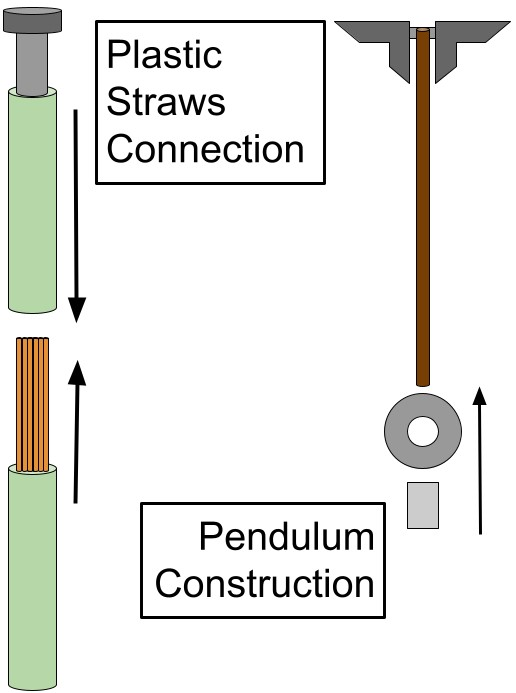
\includegraphics[width=130pt]{img/fig3.jpg}
\caption{\label{fig:3}Assembling structure and TMD}
\vspace{-10pt}
\end{figure}


For the TMD, I constructed a metal pendulum made out of old wire hanging on a screw tightened together with $90^{\circ}$ metal mantles to cause friction (hence damping) when the TMD swings \autocite{lourenco}. To modify the mass $m_p$, I will place standard $5g$ circular metal nuts into the wire, then fix them in place using a plastic slider that tightens around the wire. Finally, I had to find the constant value for the natural frequency of the swaying structure $(f)$ to match it with the frequency of the pendulum so that both oscillate in the same time period, thus creating damped simple harmonic motion. To do this, I offset the structure by 5.00cm, released, and measured the period, $T=(0.700\pm 0.005)s$, then solved for frequency, $f=\frac{1}{0.700s}=(1.43\pm0.01)Hz$. To synchronise the frequency of the TMD with $f$, I modified the length of the pendulum using $L=\frac{g}{4\pi^2f^2}$, derived from the period of a pendulum. $$\frac{1}{f}=2\pi\sqrt{\frac{L}{g}} \rightarrow L=(0.122\pm0.002)m$$ where $g$ is the gravitational constant ($9.81 \frac{m}{s^2}$). Hence, the TMD will oscillate at the same frequency as the structure but in the other direction, thereby tuning the mass damper \autocite{connor}. Lastly, I will attach a Raspberry Pi microcomputer to the top of the structure where I will measure acceleration using the SenseHat accelerometer sensor, where I will program a script to collect and store the data.

\subsection{Variables}

\textbf{Independent variable: }
Mass of the Tuned Mass Damper $(m_p)$. Modified with metal nuts. Increments over: 5, 10, 15, 20, 25, 30, 35, and 40 grams.
\\ \\
\textbf{Dependent variable:}
Second crust of structure's acceleration (maximum acceleration in second oscillation) $(a_2)$.
\\ \\
\textbf{Controlled Variables:}
\\ \underline{Initial displacement} $\Delta d_1$ of the top of the structure. Must stay constant to simulate constant magnitude of earthquake in each trial. If inconsistent, initial acceleration will vary, resulting in different $a_2$ values throughout the trials. I will control this by releasing the structure from the same distance of 5.00cm (measured by placing top of structure parallel to wall). Moreover, I can anticipate minor inaccuracies because they will average out over the multiple trials.
\\ \\ \underline{Structure’s material and dimensions.} The structure itself should stay durable by not bending the straws nor damaging its structural integrity. A change in structural integrity could cause additional damping which would skew the damping effect, which would decrease $a_2$ irrespective of $m_p$. I can anticipate this problem by monitoring the consistency of $a_2$ throughout the trials. I will control this variable using durable materials and not overloading the TMD (max weight 40g).

\subsection{Materials}

% Please add the following required packages to your document preamble:
% \usepackage[table,xcdraw]{xcolor}
% If you use beamer only pass "xcolor=table" option, i.e. \documentclass[xcolor=table]{beamer}

\begin{table}[h]
\begin{tabular}{lllll}
\multicolumn{1}{c}{\cellcolor[HTML]{343434}{\color[HTML]{FFFFFF} \textbf{Material}}}                                                                        & \multicolumn{1}{c}{\cellcolor[HTML]{343434}{\color[HTML]{FFFFFF} \textbf{Properties}}}                                                                                                   &  &  &  \\
\cellcolor[HTML]{EFEFEF}{\color[HTML]{000000} 8x Metal nuts}                                                                                                & \cellcolor[HTML]{EFEFEF}{\color[HTML]{000000} Weighing 5g each}                                                                                                                          &  &  &  \\
\cellcolor[HTML]{C0C0C0}{\color[HTML]{000000} 8x plastic straws}                                                                                            & \cellcolor[HTML]{C0C0C0}{\color[HTML]{000000} Measuring 15cm each}                                                                                                                       &  &  &  \\
\cellcolor[HTML]{EFEFEF}{\color[HTML]{000000} 32x wooden toothpicks}                                                                                        & \cellcolor[HTML]{EFEFEF}{\color[HTML]{000000} 4x to attach straws together}                                                                                                              &  &  &  \\
\cellcolor[HTML]{C0C0C0}{\color[HTML]{000000} 1x copper wire}                                                                                               & \cellcolor[HTML]{C0C0C0}{\color[HTML]{000000} Rigid; $(12.2\pm0.2)cm$ long}                                                                                                                        &  &  &  \\
\cellcolor[HTML]{EFEFEF}{\color[HTML]{000000} 10x metal screws}                                                                                             & \cellcolor[HTML]{EFEFEF}{\color[HTML]{000000} \begin{tabular}[c]{@{}l@{}}4x for base, 4x for ceiling, 2x for pendulum, \\ 1x for fixing base to platform\end{tabular}}                   &  &  &  \\
\cellcolor[HTML]{C0C0C0}{\color[HTML]{000000} 3x synthetic wood planks}                                                                                     & \cellcolor[HTML]{C0C0C0}{\color[HTML]{000000} \begin{tabular}[c]{@{}l@{}}2x 5cm by 5cm for base and ceiling of structure\\ 1x 15cm by 15cm for platform\end{tabular}}                    &  &  &  \\
{\color[HTML]{000000} 2x metal handle for pendulum}                                                                                                         & {\color[HTML]{000000} \begin{tabular}[c]{@{}l@{}}Right-angled piece, screwed to ceiling, with holes \\ for screw to go through, copper wire around it\end{tabular}}                      &  &  &  \\
\cellcolor[HTML]{C0C0C0}{\color[HTML]{000000} 1x adjustable slider}                                                                                         & \cellcolor[HTML]{C0C0C0}{\color[HTML]{000000} plastic slider to fix weights in place on pendulum}                                                                                        &  &  &  \\
\cellcolor[HTML]{EFEFEF}{\color[HTML]{000000} \begin{tabular}[c]{@{}l@{}}Raspberry Pi SenseHAT Accelerometer\\ wirelessly connected to laptop\end{tabular}} & \cellcolor[HTML]{EFEFEF}{\color[HTML]{000000} \begin{tabular}[c]{@{}l@{}}Sensor attached to top of structure ($\pm0.001ms^{-2}$)\end{tabular}} &  &  &
\end{tabular}
\end{table}


\section{Method}


\begin{figure}[h]
\centering
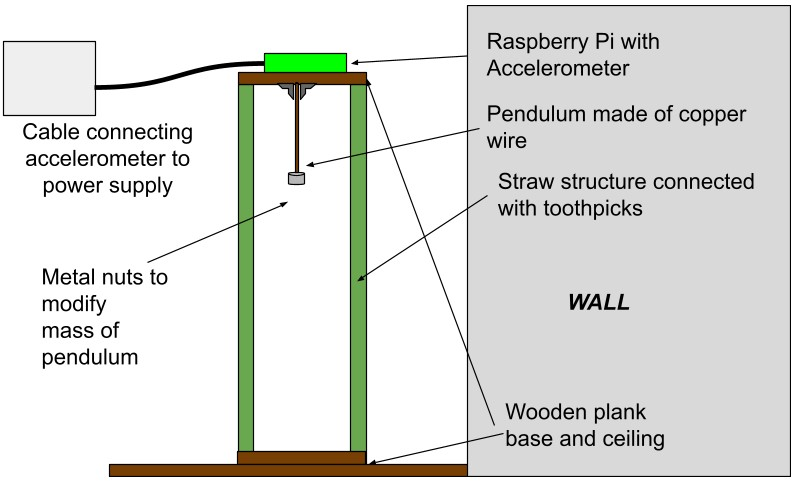
\includegraphics[width=330pt]{img/fig4.jpg}
\caption{\label{fig:4}Experiment Setup}
\end{figure}

\begin{enumerate}

\item Ensure that the structure dimensions are not altered by checking if the structure is visually deformed or bent. Tighten the straws together if loose to increase consistency and reliability of data. If the straws bend or the structure is leaning to one side, then replace with new straws.
\item Connect to Raspberry Pi through wireless Secure Shell Connection from laptop through terminal \autocite{ssh}. Run custom accelerometer reader program to begin gathering raw data.
\item Displace the top of the structure until it reaches the wall, which by design of the platform is exactly $5.00cm$ away, removing likely human error possible when using ruler to displace thus maximizing accuracy of results. Ensure that it is fully in contact with wall before releasing to maintain $\Delta d_1$ precise and accurate for control variables to be consistent across trials.

\item Release the structure, avoid applying an additional force in the form of a push by letting go of structure gently and quickly. This maximizes accuracy in the data because the initial acceleration is constant across trials.
\item After the structure oscillates back and forth approximately twice, stop recording program, download data to computer from Raspberry Pi microcomputer via connection, then disconnect.
\item Record the measure of the amplitude in the acceleration graph ($a_2$ in $ms^{-2}$) during its second period of oscillation displayed using my custom Python program using data visualization libraries. Use highest recorded acceleration during second period of oscillation in order to minimize human error when reading the data thus maximizing accuracy.
\item Repeat steps 1 to 6 for trial 2, 3, 4, 5, 6, 7.
\item Detach slider from pendulum, attach another metal nut to the bottom of the pendulum to increment the mass through the values 5, 10, 15, 20, 25, 30, 35, and 40 grams. Tighten the slider to ensure they do not fall once fixed in place.
\item Repeat steps 1-8 for each increment in step 8.

\end{enumerate}

\section{Risk assessment and ethical concerns}
\begin{description}
    \item[Ethical and Safety Concerns] This experiment is free of ethical concerns because it does not involve other beings and is free of safety concerns as it is not dangerous for any parties involved.
    \item[Environmental Concerns] All materials are reusable except for the plastic straws which will be properly recycled when disposed of, implying limited environmental concerns. Therefore, this experiment has no significant risk or ethical concerns associated with it and carefully approaches any environmental concerns.
\end{description}

\section{Data and Analysis}

\begin{table}[H]
\begin{tabular}{ccccccccc}
\rowcolor[HTML]{FFFFFF}
\cellcolor[HTML]{EFEFEF}{\color[HTML]{9B9B9B} }       & \multicolumn{7}{c}{\cellcolor[HTML]{FFFFFF}\begin{tabular}[c]{@{}c@{}}Acceleration at Second Crest of Acceleration Graph\\ $ms^{-2}$\\ $\Delta ms^{-2} = \pm 0.001$\end{tabular}} & \cellcolor[HTML]{EFEFEF}                                              \\
\rowcolor[HTML]{EFEFEF}
\begin{tabular}[c]{@{}c@{}}Mass ($m_p$)\\ g\\ $\Delta g=\pm 0.01$\end{tabular} & Trial 1              & Trial 2              & Trial 3              & Trial 4              & Trial 5             & Trial 6             & Trial 7             & \begin{tabular}[c]{@{}c@{}}Mean Acceleration ($a_2$)\\ $ms^{-2}$\end{tabular} \\
5.00                                                     & 2.013                & 2.019                & 2.022                & 2.015                & 2.023               & 2.021               & \textbf{2.054}               & 2.019 $\pm0.005$                                                                \\
\rowcolor[HTML]{EFEFEF}
10.00                                                    & 1.856                & 1.851                & 1.862                & 1.854                & 1.861               & 1.865               & 1.858               & 1.858 $\pm0.007$                                                                 \\
15.00                                                    & 1.733                & 1.735                & 1.737                & 1.739                & 1.730                & 1.741               & 1.729               & 1.735 $\pm0.006$                                                                 \\
\rowcolor[HTML]{EFEFEF}
20.00                                                    & 1.632                & 1.631                & 1.630                 & 1.634                & 1.625               & 1.634               & 1.642               & 1.633 $\pm0.008$                                                               \\
25.00                                                    & 1.529                & 1.530                 & 1.532                & 1.520                 & 1.519               & 1.531               & 1.533               & 1.528 $\pm0.007$                                                                \\
\rowcolor[HTML]{EFEFEF}
30.00                                                    & 1.450                & 1.453                 & 1.444                & 1.439                & 1.437               & 1.439               & 1.437               & 1.443 $\pm0.008$                                                                \\
35.00                                                    & 1.401                & 1.412                & 1.396                & 1.398                & 1.395               & 1.409               & 1.404               & 1.402 $\pm0.008$                                                                \\
\rowcolor[HTML]{EFEFEF}
40.00                                                    & 1.385                & 1.381                & 1.369                & 1.384                & 1.376               & 1.380                & 1.382               & 1.380 $\pm0.008$
\end{tabular}
\caption{\label{tbl:1}Raw data showing mass(g) and acceleration($ms^{-2}$)}
\end{table}

% Please add the following required packages to your document preamble:
% \usepackage[table,xcdraw]{xcolor}
% If you use beamer only pass "xcolor=table" option, i.e. \documentclass[xcolor=table]{beamer}


Collected data (in Table 1) is gathered to four significant figures with uncertainty $\pm0.001ms^{-2}$. The mean acceleration is calculated in the rightmost column by adding all trials and dividing by 7, with uncertainty calculated using $\frac{(Range)}{2}$. The calculated uncertainty is larger than the device's uncertainty, which reflects human error caused by minor variations in control variables, although it is low as it remains at three decimal places and is averaged out throughout the 7 trials for increased precision.
\\


However, trial 7 of the first increment highlighted in bold, $2.054$, is an \textbf{outlier} as it falls above the upper limit of the interquartile range, $$1.5\times IQR+Q_3=1.5\times0.008+2.023=\underline{2.035}$$ Therefore, it will not be used in any calculations as to maintain high precision throughout the analysis. This could have been caused by an additional force placed onto the structure when releasing it from $\Delta d_1$. There are no other outliers in the data.
\\


Figure 5 is an example of Trial 2, $m_p=5.00g$, of the raw data measured using the Raspberry Pi SenseHAT, visualised using the MatPlotLib and Numpy packages in a custom Python script I made displaying raw data gathered from the accelerometer \autocite{matplotlib, numpy, python}. The release of the structure is shown in the initial spike, after which follows dampened SHM motion. $a_2$ is gathered by taking the value at the crest of the second period of oscillation, which corresponds with the maximum value at the second peak on the acceleration graph (example: $a_2$ occurs at $t=1.49$ with acceleration $2.019ms^{-2}$. The pattern produced resembles damped simple harmonic motion, which further validates that the experiment was set up properly to simulate an earthquake's effect on a building.

\begin{figure}[h]
\centering
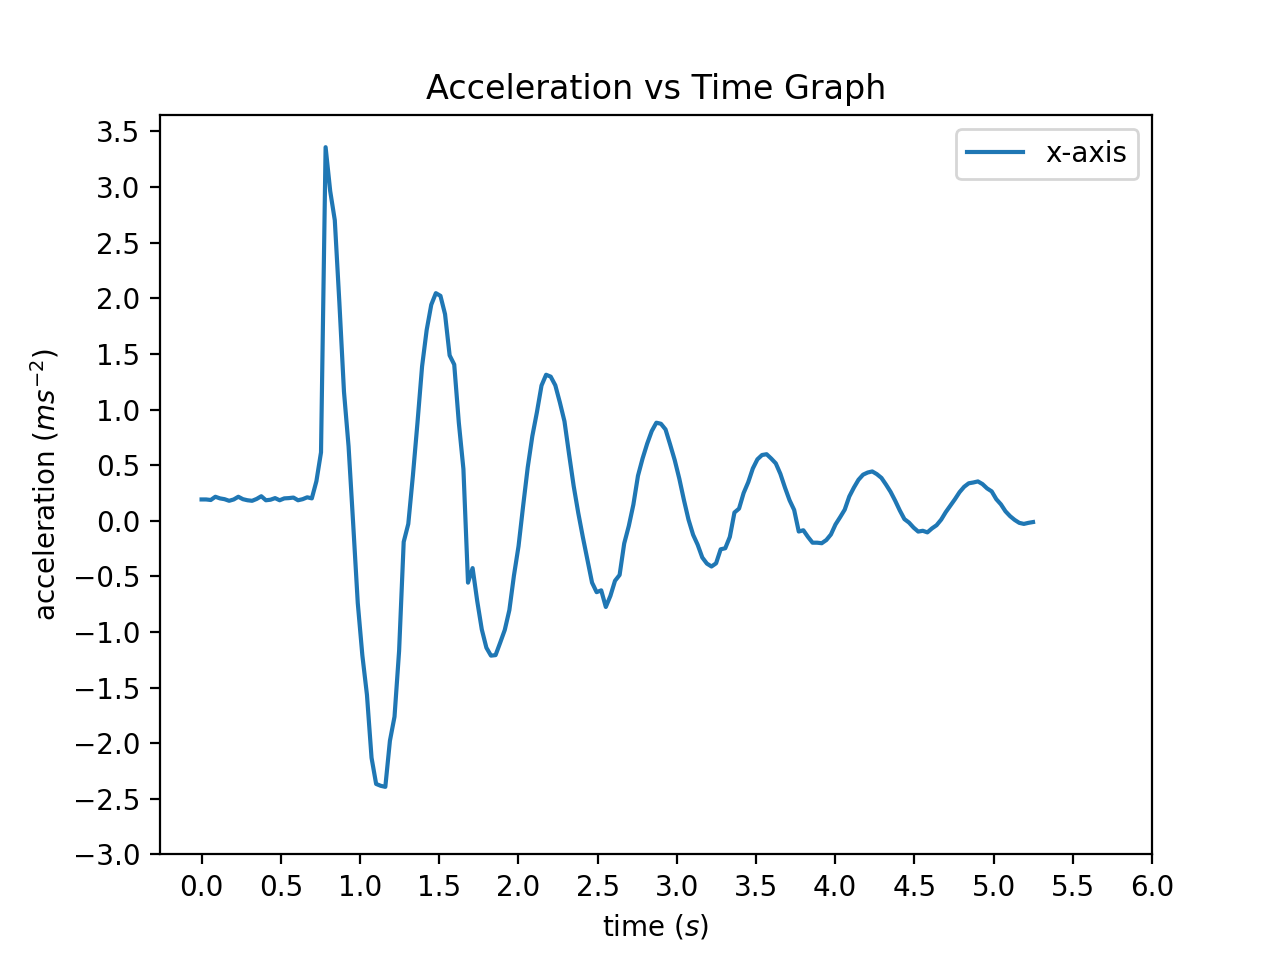
\includegraphics[width=330pt]{img/example_trial.png}
\caption{\label{fig:5}Trial 2 Raw Accelerometer Data Plotted Using Matplotlib script}
\end{figure}

With the $a_2$ values retrieved from the acceleration versus time graph of each trial and increment, the data can now be processed from acceleration to \% of dissipated mechanical energy.

\newpage
\subsection{Processing Data}

\begin{table}[h]
\begin{tabular}{cccccccccc}
\rowcolor[HTML]{FFFFFF}
\cellcolor[HTML]{EFEFEF}{\color[HTML]{9B9B9B} }       & \multicolumn{8}{c}{\cellcolor[HTML]{FFFFFF}\begin{tabular}[c]{@{}c@{}}Percentage of Dissipated Mechanical Energy $\zeta$\\ $\%$\end{tabular}}                                                                                                                                                                                                                                                                               & \cellcolor[HTML]{EFEFEF}                                 \\
\rowcolor[HTML]{EFEFEF}
\begin{tabular}[c]{@{}c@{}}Mass ($m_p$)\\ g \\ $\Delta g=\pm 0.01$\end{tabular} & Trial 1                                          & Trial 2                                          & Trial 3                                          & Trial 4                                          & Trial 5                                          & Trial 6                                          & Trial 7                                          & \begin{tabular}[c]{@{}c@{}}$\zeta$ Uncertainty\\ $\Delta \%$\end{tabular} & \begin{tabular}[c]{@{}c@{}}Mean $\zeta$\\ $\%$\end{tabular} \\
5.00                                                  & 75                                             & 75                                             & 75                                             & 75                                             & 75                                             & 75                                             & \cellcolor[HTML]{C0C0C0}                         & $\pm 1$                                                          & 75 $\pm 1$                                                     \\
\rowcolor[HTML]{EFEFEF}
10.00                                                 & 79                                             & 79                                             & 79                                             & 79                                             & 79                                             & 79                                             & 79                                             & $\pm 1$                                                          & 79  $\pm 1$                                                    \\
15.00                                                 & 82                                             & 82                                             & 82                                             & 81                                             & 82                                             & 81                                             & 82                                             & $\pm 1$                                                          & 82 $\pm 1$                                                     \\
\rowcolor[HTML]{EFEFEF}
20.00                                                 & 83.7                                             & 83.7                                             & 83.7                                             & 83.6                                             & 83.8                                             & 83.6                                             & 83.5                                             & $\pm 0.9$                                                          & 83.6  $\pm 0.9$                                                    \\
25.00                                                 & 85.7                                             & 85.6                                             & 85.6                                             & 85.8                                             & 85.8                                             & 85.6                                             & 85.6                                             & $\pm 0.8$                                                          & 85.7 $\pm 0.8$                                                     \\
\rowcolor[HTML]{EFEFEF}
30.00                                                 & 87.1                                             & 87.0                                             & 87.2                                             & 87.3                                             & 87.3                                             & 87.3                                             & 87.3                                             & $\pm 0.7$                                                          & 87.2 $\pm 0.7$                                                     \\
35.00                                                 & \multicolumn{1}{r}{88.0}                         & \multicolumn{1}{r}{87.8}                         & \multicolumn{1}{r}{88.0}                         & \multicolumn{1}{r}{88.0}                         & \multicolumn{1}{r}{88.1}                         & \multicolumn{1}{r}{87.8}                         & \multicolumn{1}{r}{87.9}                         & $\pm 0.7$                                                          & 87.9 $\pm 0.7$                                                     \\
\rowcolor[HTML]{EFEFEF}
40.00                                                 & \multicolumn{1}{r}{\cellcolor[HTML]{EFEFEF}88.2} & \multicolumn{1}{r}{\cellcolor[HTML]{EFEFEF}88.3} & \multicolumn{1}{r}{\cellcolor[HTML]{EFEFEF}88.5} & \multicolumn{1}{r}{\cellcolor[HTML]{EFEFEF}88.2} & \multicolumn{1}{r}{\cellcolor[HTML]{EFEFEF}88.4} & \multicolumn{1}{r}{\cellcolor[HTML]{EFEFEF}88.3} & \multicolumn{1}{r}{\cellcolor[HTML]{EFEFEF}88.3} & $\pm 0.7$                                                          & 88.3 $\pm 0.7$
\end{tabular}
\caption{\label{tbl:2}Processed data showing mass(g) and percentage of dissipated mechanical energy($\%$)}
\end{table}


The Percentage of Dissipated Mechanical Energy is calculated using $\zeta=\frac{\Delta d_1^2-(\frac{a_2}{4\pi^2f^2})^2}{\Delta d_1^2} \times 100\%$ \\
and then formatted to the decimal places of its uncertainty, seen in Table 2.
For example, trial 1 at $m_p=5.00g$ is calculated using:
$$\zeta=\frac{0.05^2-(\frac{2.013}{4\pi^2\times1.43^2})^2}{0.05^2} \times 100\% = 75.\underline{13}=75 \% \; \textrm{  (no decimal place)}$$

To calculate the uncertainty of $\zeta$, we can apply the uncertainty rules for addition, multiplication, and exponents of uncertainties to derive an equation for uncertainty. Following these rules, we first ignore all terms without uncertainties, producing the modified equation:
$$\zeta \rightarrow (\frac{100}{16\pi^4\Delta {d_1}^2}) \times \frac{(a_2 \pm \Delta a_2)^2}{(f \pm \Delta f)^4}$$
Then we apply the uncertainty rules to this equation, producing the final equation for the uncertainty of $\zeta$, defined as $\Delta \zeta$:
$$ \therefore \Delta \zeta = (\frac{100}{16\pi^4\Delta {d_1}^2})\times(\frac{2a_2 \Delta a_2}{f^4} + \frac{4{a_2}^2\Delta f}{f^5})$$
However, the TMD's frequency varied between recorded trials. This inconsistency adds to the uncertainty of the processed data because the equation for $\zeta$ assumes a constant frequency $f$. The values varied between $1.41Hz$ and $1.45Hz$, therefore the uncertainty of the frequency will be modified to $\Delta f = \frac{(Range)}{2} = \frac{1.45-1.41}{2} = 0.02Hz$. Now, the equation for $\Delta \zeta$ can be substituted with the following values:
$$f \pm \Delta f = (1.43 \pm 0.02)Hz, \; \; \Delta a_2 = \pm 0.001ms^{-2}, \; \; \Delta d_1 = 0.05m$$


Then, to calculate the uncertainty of the same example data point as before:
$$\Delta \zeta = (\frac{100}{16\pi^40.05^2})\times(\frac{2\times2.013 \times0.001}{1.43^4} + \frac{4\times2.013^2\times0.02}{1.43^5})=1.4\% = 1\% \; \textrm{  (one significant figure)}$$



The uncertainty decreases over higher values of $m_p$ since acceleration decreases, although it is much larger than in the raw data since acceleration is squared and the uncertainty of the frequency is considered. Consequently, the first three increments are formatted to zero decimal places to account for the larger uncertainty, whereas the later trials are formatted to one decimal place because of lower uncertainty. While it may seem like precision is lost because of one less significant figure, the differences across means are significantly larger in the first three increments which accounts for the increase in uncertainty. Therefore, precision is still maintained. Additionally, the uncertainty turns out to equal the same value across each increment, hence it is a column in the data table to improve readability. The mean percentage of dissipated mechanical energy is calculated by averaging the trials, however, since uncertainty is constant throughout each trial, the same uncertainty will be used in the mean. This ensures that accuracy is not artificially increased by using the mean of the data.
\\



Moreover, standard deviation of the processed data yields $\sigma =0.1\%$ or less for each increment of $m_p$ (hence it is not shown in a data table to avoid repetition). This value is very low, thus further validating the precision of the processed data. This data can now be graphed to understand its trend.


\begin{figure}[h]
    \centering
    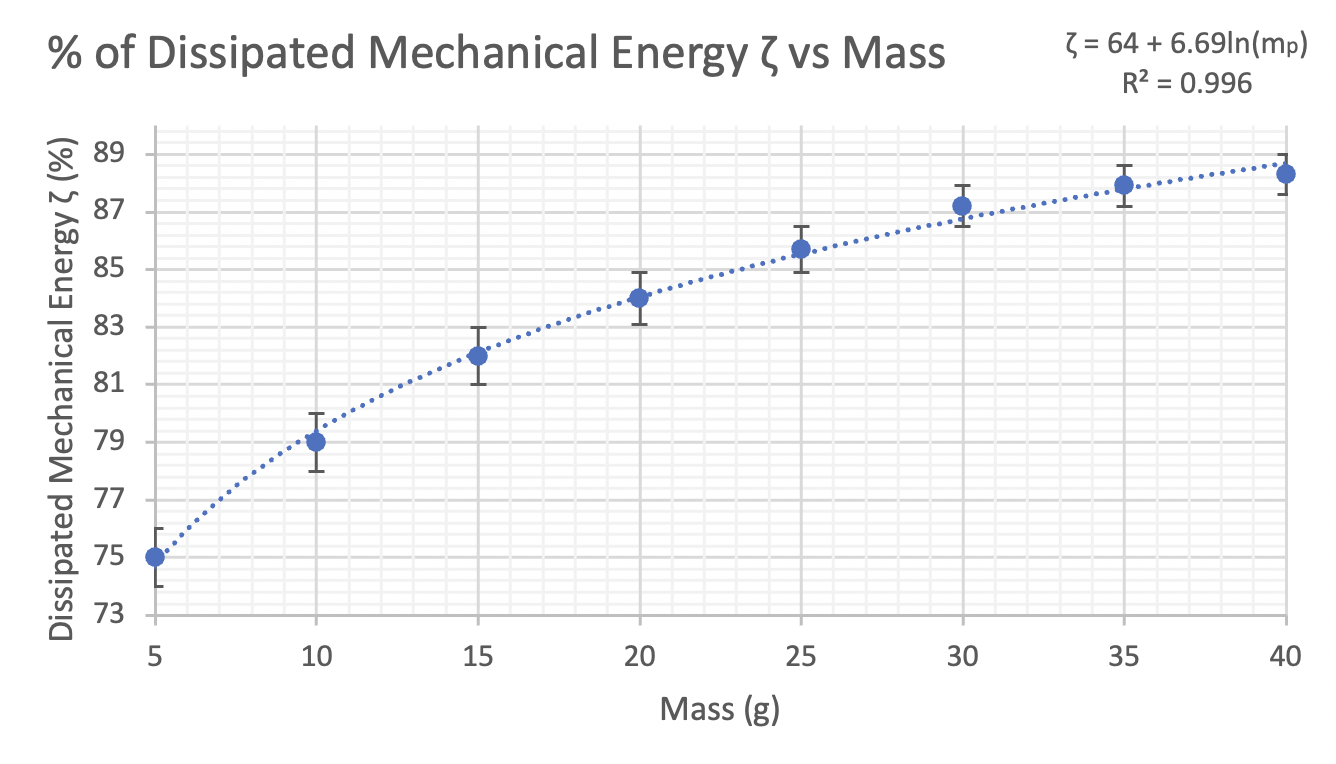
\includegraphics[width=0.9\textwidth]{img/graph1.png}
    \vspace{-20pt}
    \caption{Graph of \% of Dissipated Mechanical Energy vs Mass}
    \label{fig:6}
\end{figure}

The processed data follows a strong logarithmic relationship, as it takes an exponentially increasing amount of mass to dissipate larger percentages of mechanical energy. The logarithmic correlation relates $\zeta = k + A\ln{m_p}$, where $k$ and $A$ are constants. Using software, the line of best fit is $$\zeta = 64 + 6.69\ln m_p$$ with a high coefficient of determination of $R^2 = 0.996$, which indicates that the line of best fit accurately resembles the data. Moreover, the line of best fit passes through every error bar, which reflects that the data is precise. This would not have been the case if the processed data uncertainty would have been calculated using the mean of the trials, which reflects how accounting for discrepancy in frequency was important and properly taken into account in the previous section.\\


The equation for $\zeta$ can be rearranged to solve for the percentage of mechanical energy damped because of the change in mass which gives a better understanding on the influence of the TMD,

$$ \zeta - 64\% = E_{TMD} = 6.69 \ln m_p$$

Where $E_{TMD}$ represents the energy dissipated by the TMD. This value is proportional to $6.69 \ln m_p$, where the coefficient $6.69$ magnifies the effect of mass on $E_{TMD}$ and thus dissipates more mechanical energy.

%https://oeis.org/wiki/List_of_LaTeX_mathematical_symbols
\newpage

\section{Conclusion}

The experiment measured the acceleration during the second peak of oscillation to deduce the percentage of mechanical energy dissipated between the first two consecutive periods. The data does not support the hypothesis, which suggests a far more interesting conclusion about the nature of the damper. Although it was hypothesized that since the kinetic energy of the damper is directly proportional to the mass then it would similarly be proportional to dissipated energy, $KE_p \propto m_p \propto \zeta$, the experiment reveals that the dissipated mechanical energy is actually a logarithmic function $\zeta = k + A\ln m_p$ for some constant $k$ and $A$. By measuring $a_2$ and processing the raw data into $\zeta$ using equation 1, which using software concluded the final equation

$$\zeta (\%) = 64\% + 6.69\ln m_p$$

Firstly, this conclusion suggests that $m_p$ and $\zeta$ increase logarithmically rather than linearly, which translates into heavier TMDs providing increasingly less additional damping for larger masses. This suggests that although the kinetic energy of the TMD increases linearly with mass, less energy overall is transferred into the TMD when the mass is higher, so the TMD moves less and thus absorbs less of the mechanical energy ($KE=\frac{1}{2}m_pv^2$, velocity $v$ is smaller). Moreover, it suggests that a lot of the kinetic energy of the TMD is transferred back into the kinetic energy of the structure, because the energy is dissipated primarily through the friction of the screw on the TMD which does not entirely dissipated the TMD's kinetic energy. \\


Secondly, the constant $k=64\%$ indicates that a TMD only provides additional damping to the initial loss of internal energy through friction within the structure. This coincides with established knowledge that imperfect oscillators are damped as energy is transferred to their surroundings through heat and internal friction. Although this function is inaccurate as $m_p$ approaches 0 because $\zeta$ would approach $-\infty$, for small masses like $m_p = 1g$ the function demonstrates how a large percentage of mechanical energy is dispersed regardless of the TMD. \\


Therefore, the conclusion answers the research question in that the mass of a Tuned Mass Damper affects the dissipation of mechanical energy in an oscillating structure in a logarithmic fashion, as for increasingly larger masses, less additional energy is dissipated. Therefore, engineers would find it redundant to increase the mass past a threshold that would keep civilians safe inside a building during a skyscraper, because additional mass would not affect damping much yet would cost more to implement. Also interestingly, the experiment reveals how even a small Tuned Mass Damper can have a large effect on the dissipation of mechanical energy. Therefore, these methods should be pursued in skyscrapers that may not have much space for larger masses, because even relatively low masses can radically improve the safety of civilians in an oscillating skyscraper after an earthquake.

% deviate from hypothesis, because constant k means that there is an additional damping force on top of the TMD


% logarithmic relationship as opposed to linear indicates that not all energy is transferred to the ball into kinetic energy, so notprop, and that

\section{Further Investigation}
Further investigation into different types of dampers would assist in establishing architectural conventions that mitigate the effect of earthquakes and thereby save lives. Along with a tuned mass damper, there are other methods of damping worth investigating and comparing to the TMD to understand which one is more effective to be put in place. A tuned liquid damper, for instance, is another method of damping oscillations in buildings using sloshing liquids, but has similarly little research done on it \autocite{bozer}. It would be worth comparing these two methods, along with other damping systems, to evaluate the effectiveness of each. This would strengthen the conclusion made by this investigation as maybe other systems are less effective and therefore TMD's with increasingly higher mass are the only way to provide effective additional damping.

\section{Weaknesses and Improvements}

% Please add the following required packages to your document preamble:
% \usepackage[table,xcdraw]{xcolor}
% If you use beamer only pass "xcolor=table" option, i.e. \documentclass[xcolor=table]{beamer}
% \usepackage[normalem]{ulem}
% \useunder{\uline}{\ul}{}
\begin{table}[H]
\hspace{-1.3cm}
\begin{tabular}{
>{\columncolor[HTML]{FFFFFF}}l
>{\columncolor[HTML]{FFFFFF}}l
>{\columncolor[HTML]{ECF4FF}}l }
\hline
\multicolumn{1}{|l|}{\cellcolor[HTML]{FFFFFF}\textbf{\begin{tabular}[c]{@{}l@{}}Source of error  \\ and effect\end{tabular}}}                                                                                                                   & \multicolumn{1}{l|}{\cellcolor[HTML]{FFFFFF}\textbf{Significance for conclusion}}                                                                                                                                                                                                                                                                                                                                                                                                                                                                              & \multicolumn{1}{l|}{\cellcolor[HTML]{DAE8FC}\textbf{\begin{tabular}[c]{@{}l@{}}Improvements \\ to reduce error\end{tabular}}}                                                                                                                                                                                                                                                                                                                                                                                                                                           \\ \hline
\multicolumn{3}{|l|}{\cellcolor[HTML]{C0C0C0}{\ul Systematic errors influencing accuracy of data}}                                                                                                                                                                                                                                                                                                                                                                                                                                                                                                                                                                                                                                                                                                                                                                                                                                                                                                                                                                                                                                                                                                                                                                                                                                                                                         \\ \hline
\multicolumn{1}{|l|}{\cellcolor[HTML]{FFFFFF}\begin{tabular}[c]{@{}l@{}}Deformation of structure \\ as plastic straws slightly\\ bent forwards by the end \\ of the experiment.\end{tabular}}                                                   & \multicolumn{1}{l|}{\cellcolor[HTML]{FFFFFF}\begin{tabular}[c]{@{}l@{}}Overall could have \\ artificially increased \\ the dissipated mechanical \\ energy as trials progressed \\ skewing the data towards \\ lower values than real \\ value. Not that significant \\ because trials in each \\ increment do not get \\ progressively lower, which \\ indicates that deformation \\ did not have a large effect.\end{tabular}}                                                                                                                               & \multicolumn{1}{l|}{\cellcolor[HTML]{ECF4FF}\begin{tabular}[c]{@{}l@{}}Replace the straws with long plastic \\ beams that would offer similar rigidity\\ -flexibility but without deformation \\ because of stronger structural integrity. \\ Moreover, this would remove the need \\ for toothpicks connecting the straws, \\ which would mean that the bending \\ would be dispersed evenly across the \\ beam and therefore approximate an \\ ideal oscillating structure.\end{tabular}}                                                                             \\ \hline
\multicolumn{3}{l}{\cellcolor[HTML]{C0C0C0}{\ul Random errors influencing precision of data}}                                                                                                                                                                                                                                                                                                                                                                                                                                                                                                                                                                                                                                                                                                                                                                                                                                                                                                                                                                                                                                                                                                                                                                                                                                                                                              \\ \hline
\multicolumn{1}{|l|}{\cellcolor[HTML]{FFFFFF}\begin{tabular}[c]{@{}l@{}}Accelerometer sensor\\ on Raspberry Pi had small \\ random spikes that deviated \\ from damped simple harmonic \\ motion, seen in Figure 5 at \\ t = 1.6s\end{tabular}} & \multicolumn{1}{l|}{\cellcolor[HTML]{FFFFFF}\begin{tabular}[c]{@{}l@{}}Not largely significant\\  because the spikes are \\ small compared to the \\ amplitude of the damped \\ simple harmonic motion, \\ can be calculated with \\ standard deviation \\ between $a_2$ trial values \\ which ensured that \\ any outliers caused by \\ random spikes in sensor \\ were removed.\end{tabular}}                                                                                                                                                                                                      & \multicolumn{1}{l|}{\cellcolor[HTML]{ECF4FF}\begin{tabular}[c]{@{}l@{}}Conduct experiment with more \\ precise sensor that would be more \\ consistent when measuring acceleration.\end{tabular}}                                                                                                                                                                                                                                                                                                                                                                       \\ \hline
\multicolumn{1}{|l|}{\cellcolor[HTML]{FFFFFF}\begin{tabular}[c]{@{}l@{}}Unintentional force applied \\ by hand when releasing structure\\ from the displaced position against \\ the wall.\end{tabular}}                                        & \multicolumn{1}{l|}{\cellcolor[HTML]{FFFFFF}\begin{tabular}[c]{@{}l@{}}Largely reduced by the \\ careful methodology used \\ as the structure was \\ released from behind held \\ against a wall, although \\ this was the most significant \\ source of error and likely \\ caused the outlier in trail 7 row\\ 1. This would have artificially \\ increased the acceleration of \\ the object, as F = ma, which \\ would skew the results into \\ different initial acceleration \\ values and therefore higher \\ data gathered than real values.\end{tabular}} & \multicolumn{1}{l|}{\cellcolor[HTML]{ECF4FF}\begin{tabular}[c]{@{}l@{}}Use electro-mechanical earthquake \\ simulator that would shake the structure \\ by a set force instead of depending on \\ human contact.  Using a mechanical \\ oscillator which simulates an earthquake \\ with constant frequency and \\ displacement would greatly increase the \\ resemblance of the experiment to a real \\ earthquake, and would validate the data \\ with more precision due to increased \\ regulation over control variables and \\ no additional force.\end{tabular}} \\ \hline
\end{tabular}
\caption{\label{tbl:3}Table showing sources of error, their effect, and improvements}
\end{table}

\newpage

\section{Strengths}

% Please add the following required packages to your document preamble:
% \usepackage[table,xcdraw]{xcolor}
% If you use beamer only pass "xcolor=table" option, i.e. \documentclass[xcolor=table]{beamer}
\begin{table}[H]
\centering
\begin{tabular}{|l|l|}
\hline
\rowcolor[HTML]{9B9B9B}
\textbf{Strengths}                                                                                                                                                                                                                         & \cellcolor[HTML]{67FD9A}\textbf{Effect on Conclusion}                                                                                                                                                                                                                                                                                                                             \\ \hline
\begin{tabular}[c]{@{}l@{}}Digital sensor was used to \\ record accelerometer data.\end{tabular}                                                                                                                                           & \begin{tabular}[c]{@{}l@{}}The structure moved significantly faster than \\ a human could detect and measure, therefore \\ using a digital sensor improved the precision \\ and accuracy of the data and conclusion.\end{tabular}                                                                                                                                                 \\ \hline
\begin{tabular}[c]{@{}l@{}}Accelerometer was attached \\ to 'RPi 3' microcomputer \\ which allowed for simple \\ data extraction using a WiFi-\\ enabled secure connection \\ without need for disassembly\\ to extract data.\end{tabular} & \begin{tabular}[c]{@{}l@{}}Remote data extraction allowed me to not\\ physically interfere with the TMD structure and \\ thereby not alter any controlled variables like \\ bending, hence increasing precision.\end{tabular}                                                                                                                                                     \\ \hline
\begin{tabular}[c]{@{}l@{}}Programmed my own script \\ to process raw data into \\ visual graph.\end{tabular}                                                                                                                              & \begin{tabular}[c]{@{}l@{}}Since the raw data consisted of thousands of \\ accelerometer  snapshots, finding $a_2$ \\ would have taken large amounts of time if not \\ for my own script that visualized acceleration \\ versus time, making finding $a_2$ as simple as \\ quantitatively locating the second peak of \\ the graph, then extracting that acceleration.\end{tabular} \\ \hline
\begin{tabular}[c]{@{}l@{}}Straws reinforced with\\ toothpicks were chosen for\\ the structure.\end{tabular}                                                                                                                               & \begin{tabular}[c]{@{}l@{}}Allowed structure to bend without completely \\ falling apart, imitating the motion of real-life \\ skyscrapers. The elastic property allowed the \\ damping to be measured while maintaining \\ structural integrity, thus producing damped \\ simple harmonic motion, which is assumed \\ in the equations used for energy.\end{tabular}             \\ \hline
\end{tabular}
\caption{\label{tbl:4}Table showing strengths of the experiment and their effects}
\end{table}

% straws reinforced with toothpicks were chosen
% effect: rigidity-flexibility ratio of real building

% rigid copper wire was used to hang the mass
% effect: light so does not interfere with central mass of TMD yet rigid so does not bend or swing

\newpage
\begin{spacing}{1.5}
\printbibliography
\end{spacing}

\end{document}
